\usetikzlibrary{decorations.pathreplacing, arrows.meta, calc, positioning}

% --- 定义颜色以匹配原图 ---
% 定义一种类似原图的蓝色

\pgfkeys{/tikz/.cd,
    overall style/.style={
        semithick, % 改用半粗线，避免缩小后线条太粗
        >=Stealth,
        scale=0.4,         % <---- 在这里调整缩放比例
        transform shape,   % <---- 确保文字和线条也随之缩放
        node distance=1.5cm
    }
}
\begin{center}
    
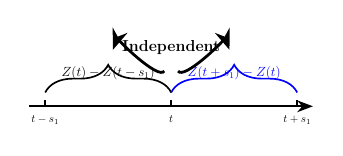
\begin{tikzpicture}[overall style]

    % --- 1. 定义坐标点 ---
    \coordinate (A1) at (0, 0);    % t - s1
    \coordinate (B1) at (4, 0);    % t
    \coordinate (C1) at (8, 0);    % t + s1

    % --- 2. 绘制数轴和刻度 ---
    \draw[->] (-0.5, 0) -- (8.5, 0);

    \foreach \pos/\label in {A1/{t-s_1}, B1/{t}, C1/{t+s_1}} {
        \draw (\pos) -- ++(0, 0.2);
        \node[below=5pt] at (\pos) {$\label$};
    }

    % --- 3. 绘制大括号和表达式 ---
    \tikzset{brace style/.style={decorate, decoration={brace, amplitude=10pt, raise=5pt}}}

    % 左侧黑色括号
    \draw[brace style] (A1) -- (B1) 
        node[midway, above=20pt, font=\large] (exprL_1) {$Z(t) - Z(t-s_1)$};

    % 右侧蓝色括号
    \draw[brace style, blue] (B1) -- (C1) 
        node[midway, above=20pt, font=\large, text=blue] (exprR_1) {$Z(t+s_1) - Z(t)$};

    % --- 4. 顶部标题和箭头 ---
    \node[above=1.5cm of B1, font=\Large\bfseries] (title_1) {Independent};

    \draw[->, line width=1pt, shorten >=5pt, shorten <=5pt] (title_1.south) to[out=240, in=70] (exprL_1.north);
    \draw[->, line width=1pt, shorten >=5pt, shorten <=5pt] (title_1.south) to[out=300, in=110] (exprR_1.north);

\end{tikzpicture}

\end{center}